\documentclass{article}

\usepackage{graphicx}% Include figure files
\usepackage{amsmath,amssymb}% Include figure files
\usepackage{dcolumn}% Align table columns on decimal point
\usepackage{bm}% bold math
\usepackage{caption}
\usepackage{subcaption}

\begin{document}

%\preprint{AIP/123-QED}

\title{Classifying Fanaroff-Riley Radio Galaxies}
\author{Josh Marsh}

\maketitle

\section{\label{sec:level1}Intoduction}

The the last few decades have seen a drastic increase
in the amount of data available to astrophysicists. As
manual methods of evaluation are often inefficient, ex-
pensive and, in many cases, highly impractical, effective
data mining techniques have often been detrimental to
many of the recent discoveries in this field.

. Give examples

In this report, we consider the classification task of radio galaxies with active nuclei within the Fanaroff-Riley
scheme. Under this scheme, galaxies that decrease in luminosity as the distance from the galactic nuclei increases are designated as FR-I, and sources that increase in luminosity towards the outer parts of the nuclei as FR-II.

. why is this problem important?

The morphological differences between the two classes
in radio images have allowed experts to classify candidates visually with a reasonable degree of accuracy. How-
ever, due to the large pool of potential candidates, this
has resulted in the discovery of only (insert number). The
citizen science project Radio Galaxy Zoo has allowed for
crowd sourcing the classification task, with (what were
the results?). While this has increased the number of
examples available to researchers, the sample size is still
small enough to make it difficult apply the state of the
art image classification methods such as deep learning.

. List attempts and results

More recently, Aniyan and Thorat showed moderate
success with convolutional neural networks, achieving a
classification accuracy of AA and AA for FR-I and FR-II
galaxies, respectively.

A core issue with classification tasks in this domain is
that it is difficult to evaluate the success of classifiers due to the lack of past studies to compare new results to. Up until recently, there was insufficient data to attempt most machine learning techniques. In essence, this means that over twenty years of machine learning methods remain
untested on the task, leaving a potential wealth of information undiscovered. In addition, the success of many
machine learning algorithms on image classification tasks
is based upon performance on optical images - radio imagery (different in what way).


\begin{figure}
 
    \begin{subfigure}[b]{0.5\textwidth}
        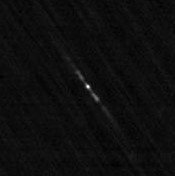
\includegraphics[width=0.5\linewidth]{FR1.jpg} 
        \caption{FR-I}
        \label{fig:subim1}
    \end{subfigure}
    \begin{subfigure}[b]{0.5\textwidth}
        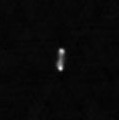
\includegraphics[width=0.5\linewidth]{FR2.jpg}
        \caption{FR-II}
        \label{fig:subim2}
    \end{subfigure}
 
    \caption{Fanaroff-Riley Radio Galaxy Examples}
    \label{fig:image2}
\end{figure}


\subsection{\label{sec:level2}Machine Learning}


Machine Learning is a broadly defined area of computer science and mathematics that allows computer algorithms to develop efficient pattern recognition methods through the iterative process of learning through the experience of performing a task to subsequently increase the performance of the algorithm. For computer vision tasks, this allows large amounts of data to dictate the feature extraction process, removing the need for experts to manually develop tailored solutions - a time-consuming and frustratingly complex endeavor. 

Supervised learning methods, which we employ primarily in this study, aim to identify probability distribution \(p \big(Y |  X \big)\) that maps an input vector \(X = \big\{x^1, x^2, x^3, ..., x^n\big\}\) to an output value \(Y\). How this is achieved depends on the machine learning method employed. 

\subsubsection{\label{sec:level3}Logistic Regression}

$$
y \big( \overrightarrow{x} \big) = p \big(z=1 \mid  \overrightarrow{x} \big) =  \sigma  \big( \overrightarrow{w}^{T}+b \big) 
$$

$$
 \sigma  \big(t\big) = \frac{1}{1+e^{-t}}
$$ 

$$
\overrightarrow{w}_{t+1} = \overrightarrow{w}_{t} -  \nabla L \big(\overrightarrow{w}_{t}\big) 
$$
 
$$
\nabla L \big(\overrightarrow{w}_{t}\big) =  -\frac{1}{N}  \sum_{ \overrightarrow{x}, z \in D } \big(z-y \big( \overrightarrow{x} \big) \big)\overrightarrow{x}

$$

\subsubsection{\label{sec:level3}Neural Networks}

. Update Heavily 

The ability of the human mind to recognize patterns in complex systems is extremely hard to match algorithmically. Artificial Neural Networks (ANN) are a computational approach of matching the functions of the human brain by mimicking synaptic connections between neurons by series of interconnected nodes organized in layers. ANNs have been successfully applied to a wide range of tasks, including character recognition, face detection, intrusion detection, speech recognition, autonomous driving, stock market prediction, and astronomy. 


\begin{figure}
\centering
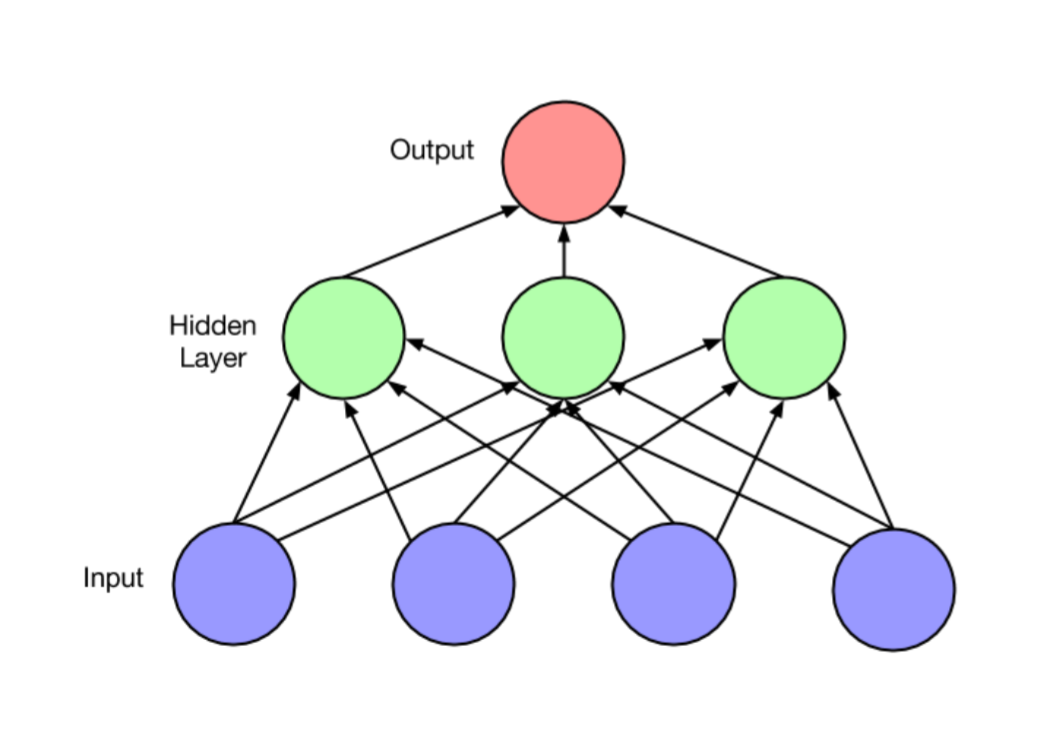
\includegraphics[width=1\linewidth]{basic_net.png}
\caption{A Basic Feed forward Neural Network.}
\label{fig:ANN}
\end{figure}

The most fundamental unit of a Neural Network is a neuron. A basic feed forward neural network consists of sets of neurons, commonly referred to as nodes, arranged into stacked layers \cite{ANN}. For a layer consisting of \(n\) individual nodes that is proceeded by a layer of \(m\) nodes, the number of connections that exist between the two layers is \(nm\). Each link between a node \(j'\) and a node \(j\), are assigned a set of trainable values, a weight \(w_{jj'}\) and a bias. Associated with each node is an activation function \(l_j(\cdot)\). The output value for node \(j\) is determined by passing the weighted sum of the inputs values through the activation function, such that:


\begin{equation}
v_j=l_j(\sum_{j'}w_{j'} \cdot v_{j'})
\end{equation}


This is represented on figure \ref{fig:node}, where the sigmoid activation function is denoted by \(\sigma\). 


\begin{figure}
\centering
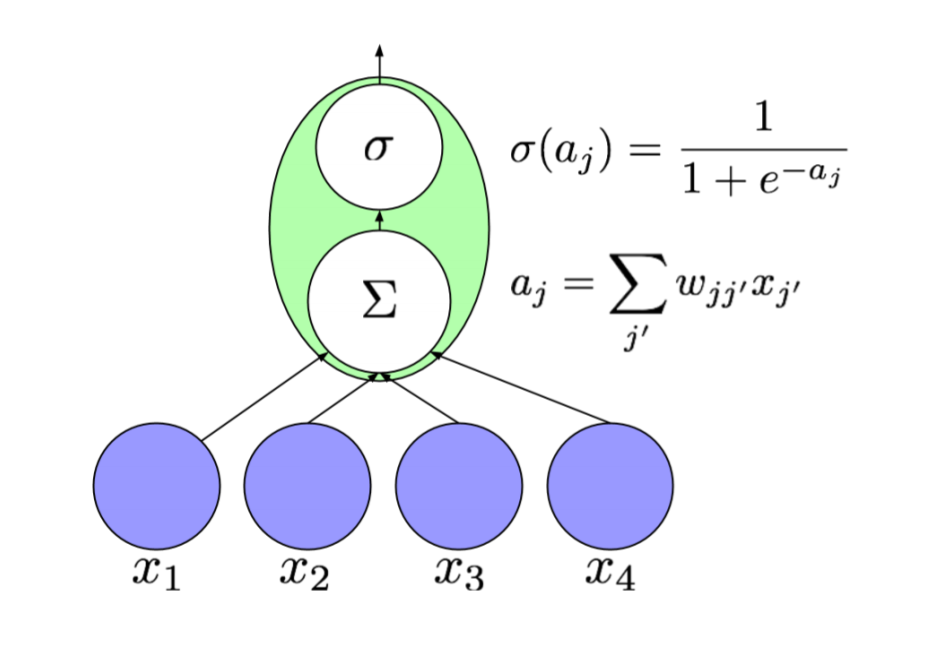
\includegraphics[width=0.8\linewidth]{node.png}
\caption{A node with a sigmoid activation function}
\label{fig:node}
\end{figure}

To train the network, input data that is labeled with a corresponding value or set of values that indicate the desired output is passed through the network. Initially, the network's weights and bias are random, thereby resulting in a random output. In order to train the network, we must find the optimal values for weights and biases that minimize the loss function, or error. This is accomplished through an optimization function. Back propagation is a highly successful gradient based optimization algorithm that operates by calculating the derivative of the loss function with respect to all the weights in the network \cite{LSTM2}.


The network learns by iterativily feeding training data through the network and updating the weights according to the loss function. Once the loss between the predicted value is close enough approximation to the correct output, when fed unseen data, the network can accurately approximate the correct output. 

\subsection{\label{sec:level2}Histogram of Orientated Gradients (HOG)}

HOG description

\section{Data and Software}

For the empirical application, we use 

(What do we use again?)

All data preparation, configuration, and management, is handled entirely within python 3.5, relying on the packages Numpy for array manipulation, Scipy for for HOG, and Skimage for it's implementations of legacy machine learning methods, such as Naïve Bayes, Random Forrest Trees, and Support Vector Machines. Neural Netowrks and Logistic Regressions were constructed using Keras, a high-level deep learning library for large scale machine learning, with Google's Tensorflow as a backend  

\section{Methodology} 
 

A core problem for quantitatively classify images is that in almost all cases there is no single feature that can be used to infer the class of the image. Human classification is a complicated and dynamic process build up through millions of years of evolution. First, we are easily able to identify if the object of interest is indeed within our field of vision. By observing an extremely minimal number of examples, we are able to intuitively infer features of importance to the object's class, subsequently allowing us to determine the class of an object by observing the degree to which each relevant feature is present, and taking a mentally weighted sum to determine which class it is most likely to belong to. It is extremely difficult to algorithmically mimic this approach.

Take the FR-I and FR-II classification task. Visually, the radio object's class is often clearly evident. Giving the FR-I galaxies frequently possess a few key features: the brightest points are always at the center of the source, the brightness usually changes more gradually, and brightness is usually inversely proportional to the distance from the sources.  FR-II radio galaxies, on the other hand, often comprise of two points that are equidistant from the source, form a strong linear correlation with the source, are often mirrored across the source, and are significantly brighter than the actual source itself. We could, in principle, take a single one of these features and build a classifier. Take the gradient for example. If the change in brightness for an FR-I source is, as a general rule, more gradual than that of an FR-II source, we can use this to determine a source's class. To illustrate: by taking the mean magnitude of the gradient for each pixel in a class for half the data, and then classifying the other half of the data based upon which value the mean gradient magnitude for each image is closest to gives an accuracy of 52.1\%. If we are to achieve an accuracy that is remotely within the range of human performance, we need to take into about all relevant features. While the degree to which these features are present in a sample can drastically vary, it is generally possible to classify a sample based upon a dynamic combination features. 

If we were to take this approach algorithmically, that is quantitatively determining the degree to which each of the relevant features exists and taking the weighted sum to determine the probability of the sample belong to either class, we would be feature engineering. This is not desirable. While theoretically capable of achieving high accuracies, many of the induvial features are extremely difficult to quantify, and are often areas of ongoing research in their own right. In addition, feature engineering is difficult to implement and is highly inflexible, making it hard to adapt to similar tasks. Due to these reasons, we instead take a machine learning based approach. 

Machine Learning techniques have been staggering successful in recent years for images classification. However, many of these algorithms, particularly state of the art methods such as convolutional neural networks, rely on vast amounts of images in order to extract useful features for classification. This makes them unsuited for tasks such as the FR-I/FR-II classification problem, where only 125 and 234 (or something) samples are known for the FR-I and FR-II classes respectively. We employ a number of methods to minimize this issue, primarily, by artificially increasing the number of samples. Using the ImageDataGenerator function in Keras, we applied a combination of random rotations, horizontal and vertical flips, horizontal and vertical translations, and zooms, allowing us to expand the dataset by a factor of one hundred. While genuine samples are preferable, this technique has been proven to be effective in the past (find sources).  Another method we employ is to convert the images into a format that allows less computationally exhaustive feature extraction. For this, we use HOG. 

\subsection{\label{sec:level2}Legacy Machine Learning Algorithms}
To establish a baseline for classification performance, we implement a Logistic Regression, Support Vector Machines (SVM), Naïve Bayes, and Random Forrest Trees (RFT).


\subsection{\label{sec:level2}Logistic Regression}

Stuff

\subsection{\label{sec:level2}Neural Network}

More stuff

\subsection{\label{sec:level2}Resnet}

Even more stuff

\subsection{\label{sec:level2}Neural Network + HOG Layer}

Your are seriously not going to belive this, but here is more stuff






\section{Results}

Results - lots of tables and graphs


\section{Discussion}

\end{document}
%
% ****** End of file aipsamp.tex ******

